\chapter{Einleitung}
Kryptographische Verfahren wie Verifikation digitaler Daten sind seit jeher wichtig für die Kommunikation auf unsicheren Kanälen.
Gerade vernetzte Kleinstrechner wie IoT-Geräte sind aufgrund ihrer geringen Leistungsfähigkeit sehr anfällig für Angreifer.
Verfahren zur Programmverifikation können dem entgegenwirken, benötigen jedoch verhältnismäßig viel Rechenleistung.
Mit Hilfe spezialisierter Hardware, die die nötigen Aufgaben effizienter ausführt, kann dieser zusätzliche Aufwand reduziert werden.
Rekonfigurierbare Prozessoren können hier Abhilfe schaffen. Sie erlauben es, kleine Hardwarebeschleuniger zur Laufzeit zu laden,
wenn sie benötigt werden und rechenintensive Aufgaben zu erledigen. Gleichzeitig müssen sie auch nicht für das spezielle
Einsatzgebiet angefertigt werden, sondern können nachträglich spezialisiert werden, was auch die Produktionskosten reduziert.
Des weiteren können die zur Verfügung gestellten Beschleuniger-Blöcke zusätzlich auch für weitere einsatzspezifische Aufgaben verwendet werden.
In dieser Arbeit wollen wir daher einen Beschleuniger für einen rekonfigurierbaren Prozessor entwickeln, der die Berechnung einer
kryptographischen Hashfunktion optimiert, dem Herzstück vieler Verifizierungsalgorithmen. Dabei wollen wir uns den i-Core als Prozessorarchitektur
zunutze machen und konkret eine SHA-3-Hashfunktion für ihn implementieren. SHA-3 ist eine relativ neue Familie an Hashfunktionen,
die auch in naher Zukunft noch viel Sicherheit verspricht und viele Probleme bisheriger Hashfunktionen verbessert.
Dazu wollen wir uns zuerst einmal den i-Core, sowie SHA-3 genauer anschauen und einen Einblick in ihre Funktionsweisen erhalten.
Danach werden wir die Impelemntierung des Beschleunigers in einem iterativen Entwurfsverfahren betrachten. Das Ziel des
Entwurfsverfahren besteht darin, einen Beschleuniger zu entwickeln, der die Anforderungen der i-Core-Architektur erfüllt
und möglichst viel seines Leistungspotentials dabei ausschöpft. Daher werden wir uns auch verschiedene Entwürfe anschauen,
um aufzuzeigen warum einige Einschnitte in der Leistungsfähigkeit notwendig sind, um die Anforderungen des i-Core zu erfüllen
und mit welchen Ansätzen trotzdem eine möglichst hohe Effizienz beibehalten werden kann. Am Ende werden wir die verschiedenen
Ansätze untereinander vergleichen und besonders gute Aspekte herausarbeiten, sowie weitere Optimierungsansätze aufzeigen,
die die Leistungsfähigkeit noch weiter steigern können. Außerdem wollen wir den entworfenen Beschleuniger mit einer
Software-Implementierung vergleichen und bestimmen wie viel effektiver der Beschleuniger gegenüber der stumpfen Software-Berechnung ist.

\chapter{i-Core}
Der icore ist ein rekonfigurierbarer Prozessor \comment{(Cite Missing)}, das bedeutet er besitzt neben den klassischen Komponenten
eines Prozessors noch eine zur Laufzeit konfigurierbare Einheit aus Hardwarebeschleunigern. 
Als Grundlage dient ein modifizierter Leon3-Kern, ein 7-Stufen-Pipeline-Prozessor basierend auf der SPARC-V8-Architektur \comment{(Cite Missing)}.
Er wird erweitert um eine sogenannte \textbf{Reconfigurable Fabric}, einen Container für fünf Beschleunigerblöcke mit Anbindung an Speicher und Registerdatei.
Wie genau diese Fabric aufgebaut ist und wie sie funktioniert schauen wir uns in Abschnitt \ref{sec:icore_arch} an.
Vorher wollen wir uns aber erstmal überlegen wofür rekonfiguruerbare Prozessoren eigentlich gut sind.
\section{Rekonfigurierbare Prozessoren}
Herkömmliche Prozessoren verfügen über einen mehr oder weniger komplexen Befehlssatz, der es ihnen erlaubt jede beliebige Berechnung durchzuführen,
indem die gewünschte Rechenoperation in mehrere vom Befehlssatz unterstützte Operationen aufgeteilt wird. Dadurch sind sie extrem flexibel.
Für rechenintensive Aufgaben, bei denen komplexere Operationen sehr oft ausgeführt werden müssen, ist dieser Ansatz jedoch nachteilig,
da der Prozessor viel Zeit benötigt, um diese komplexen Operationen zu berechnen. Um dem Abhilfe zu verschaffen, wird spezializsierte Hardware
wie zum Beispiel Grafikkarten, Netzwerkkarten oder FPGAs (siehe Abschnitt \ref{sec:fpga}) eingesetzt, die besonders effizient eine bestimmte Art von Aufgabe erfüllen.
Durch die fortschreitende Digitalisierung und Vorstöße in Bereichen wie der Industrie 4.0 oder dem Internet der Dinge (IoT) wächst der Bedarf an Kleinstrechensystemen,
die für den konkreten Anwendungszweck spezielle Aufgaben übernehmen können. Diese müssen vor allem energieeffizient, klein und günstig in der Produktion sein
und müssen dabei trotzdem auch in der Lage sein komplexere Aufgaben teilweise sogar in Echtzeit erfüllen zu können.
Ein rekonfigurierbarer Prozessor bietet hier die Vorteile der hohen Flexibilität eines normalen Prozessors und verbindet sie mit der hohen Spezialisierbarkeit von FPGAs,
indem er mehrere kleine Blöcke an vom Entwickler konfigurierbare Logikblöcke bereitstellt, die mit speziellen Prozessorinstruktionen gesteuert werden können.
Auf diese Weise können auch sehr spezielle Anwendungen von Off-The-Shelf Hardware erfüllt werden, was die Produktionskosten gegenüber Spezialanfertigungen,
sowie den Energieverbrauch und den Bedarf an Rechenleistung gegenüber klassischen Prozessoren reduziert.

\subsection{FPGA}
\label{sec:fpga}
\textbf{Field Programmable Gate Arrays} (FPGAs) sind integrierte Schaltkreise, die von sich aus keine genaue Funktion implementieren. Stattdessen muss erst eine Schaltung "geladen" werden.
Auf der kleinsten Ebene bestehen sie aus Logikblöcken und Verbindungsstrukturen. In einen Logikblock kann von außen eine boolsche Funktion "einprogrammiert" werden. Dabei macht man sich zu Nutze,
dass eine n-stellige boolsche Funktion durch einen $2^n$-Bit Vektor codiert werden kann. In Abb. \comment{\ref{fig:fpga_lut}} ist zum Beispiel die Funktion $f = A \vee (B \wedge \neg C)$ dargestellt.
Der 8-Bit Ergebnisvektor wird in SRAM-Speicherzellen gehalten und durch einen 8-zu-1-Multiplexer kann mit $A$, $B$ und $C$ das entsprechende Ergebnisbit ausgewählt werden. Diese Schaltung wird Lookup Table (LUT) genannt.
Eine Logikzelle enthält neben einem solchen Lookup Table meist noch ein Flip-Flop, sodass das Ergebnis gespeichert oder direkt ausgegeben werden kann.


\section{icore-Architektur}
\label{sec:icore_arch}

\section{Erweiterung Dynamic Execution}

\chapter{SHA-3}
\documentclass{article}
\usepackage{xcolor}
\newcommand\todo[1]{\textcolor{red}{#1}}

\begin{document}

\section{SHA-3}

Unter "Secure Hash Algorithm" (SHA) versteht man eine Familie kryptographischer Hashfunktionen, die von dem US-amerikanischen "National Institute of Standards and Technology" standartisiert werden \todo{oder spezifiziert?}.
Eine solche kryptographischen Hashfunktion bildet eine Eingabe beliebiger Länge auf einen kurzen Zahlenwert fester Länge ab, wobei die Ausgabe für einen Angreifer von echtem Zufall ununterscheidbar sein soll.


\subsection{Sicherheitseigenschaften}

\subsubsection{Kollisionsresistenz}
Eine Hashfunktion H(x) gilt als kollisionsresistent, wenn ein Angreifer nur mit vernachlässigbarer Wahrscheinlichkeit zwei verschiedene Eingaben M und M' findet, die auf den gleichen Hashwert abgebildet werden (H(M) = H(M')).

\subsection{Aufbau}
Typischerweise besteht eine solche Hashfunktion aus einer Kompressionsfunktion, die einen Eingabeblock auf eine kleinere Ausgabe abbildet. Die Eingabenachricht wird in mehrere Blöcke aufgeteilt, worauf die Kompressionsfunktion so
oft angewendet wird, bis die gewollte Ausgabegröße erreicht ist. Die Art und Weise wie die Kompressionsfunktion verwendet wird, wird Betriebsmodus genannt. Der am weitesten verbreitete Betriebsmodus ist die Merkle-Damgard-Konstruktion.
Sie hat die schöne Eigenschaft, dass sie die Kollisionsresistenz der Kompressionsfunktion auf die entstehende Hashfunktion überträgt. Das gilt jedoch leider nicht für alle Sicherheitseigenschaften, die man sich von einer Hashfunktion wünscht.
So lassen sich zum Beispiel Angriffe gegen Message Authentication Codes (MACs) konstruieren, die auf der Merkle-Damgard-Konstruktion aufbauen.

Während SHA-0, SHA-1 und SHA-2 diese Merkle-Damgard-Konstruktion verwenden, setzt SHA-3 auf einen anderen Betriebsmodus, die Schwammkonstruktion. Sie verwendet keine Kompressionsfunktion, sondern lediglich eine Permutation oder Transformation
wobei der Ergebnisraum genau der Größe des Werteraums entspricht. Besonders hervorzuheben ist hier, dass die entstehende Hashfunktion kollisionsresistent ist, wenn die verwendete Permutation ununterscheidbar von einem Zufallsorakel ist,
selbst wenn sie leicht invertierbar ist.

\section{Sicherheit gegen Quantenalgorithmen}
Wenn auch nicht bewiesen, so wird vemutet, dass Quantencomputer deutlich mächtiger sind als konventionelle Rechensysteme. Zwar ist unwahrscheinlich, dass in den nächsten Jahren Systeme mit genügend Rechenleistung auftauchen,
trotzdem sollten aber neue Verfahren gegen solche Angreifer standhalten können. Bisher wurde gezeigt, dass die Schwammkonstruktion auch für Quantenalgorithmen nicht vom Zufall unterscheidbar ist.

\section{Aufbau von SHA-3}
\subsection{Keccak-Permutationsfuktion}
KECCAK-p[b, nr] ist eine Funktionenfamilie, die über die beiden Parameter b und nr definiert ist. Zur Kryptoanalyse wird die 

\subsection{Schwammkonstruktion}

\end{document}

\chapter{Implementierung}
\input{chapters/optimierungsansaetze.tex}
\newpage
\section{Erste Iteration}
\subsection{Entwurfsziele}

Die Architektur gibt eine maximale Größe von 1600 LUTs für seine Beschleunigerblöcke vor und ein Beschleuniger kann aus maximal 5 solcher Blöcke bestehen.
Weiterhin permutiert die Keccak-Funktion ein 1600 Bit breites Feld, wobei jedes Bit von vielen anderen Bits an verschiedenen Stellen im Feld abhängt.
Da die verschiedenen Blöcke nicht beliebig miteinander kommunizieren können, sondern nur über eine taktsynchrone Schnittstelle mit sehr begrenzter Bandbreite,
folgt aus den beiden Beobachtungen die Vermutung, dass ein guter Beschleuniger aus so wenig Blöcken wie möglich besteht.
Ziel des ersten Entwurfs war daher einen Beschleuniger zu entwickeln, der die Keccak-Permutation so schnel wie möglich in einem Block berechnet.
Dabei war es erlaubt die Größenbeschränkung von 1600 LUTs in einem sinnvollen Maß zu überschreiten um daraufhin das Optimierungspotential des Entwurfs zu untersuchen
und nach und nach die Größe zu reduzieren, bis schließlich das Größenlimit eingehalten wird.
So sollten zum Beispiel nicht einfach alle 24 Runden in einem Takt über eine riesige kombinatorische Schaltung berechnet werden,
da selbst für eine einzelne Runde die 1600 LUTs für die 1600 Bit Ausgabe schon kritisch sind.
Weil sich die einzelnen Runden voneinander nur in einem Rundenindex unterscheiden, der sich in einer 64-Bit Konstanten in der Iota-Funktion manifestiert,
hätte man eine um Größenordnungen zu große Schaltung mit sehr viel repetetiver Logik.

\subsection{Aufbau}
Daher Bestand der erste Entwurf direkt aus einer kombinatorischen Schaltung, die eine komplette Runde berechnet sowie einem Register,
das die Ausgabe dieser Schaltung speichert und wieder als Eingabe bereit stellt.
[Bild hier + Beschreibung]

\subsection{Bewertung}
Letztendlich besteht der erste Entwurf aus \comment{circa 3500 LUTs, Zahl muss noch präzisiert werden} ohne Kommunikationslogik.
Die Zahl setzt sich aus ungefähr 1600 LUTS für das Speichern der Daten zusammen und der Rest wird von der kombinatorischen Rundenfunktion benötigt.
Das ist zwar noch etwa doppelt so groß wie das finale Design am Ende sein soll, aber mit ein paar Anpassungen kann die größe potentiell weiter reduziert werden.

\subsection{Optimierungsansätze}
Der wohl naheliegendste Gedanke ist den Datenspeicher zu reduzieren, da er mit seinen 1600 LUTs bereits das gesammte Budget alleine benötigt.

\subsubsection{Aufspalten der Rundenfunktion}
Um die Rundenfunktion in mehrere Teile aufteilen zu können, ist eine genauere Untersuchung der Funktion selbst notwendig um Teie ausfindig zu machen,
die unabhängig voneinander berechnet werden können. Das Aufteilen in die gleichen Teilfunktionen, aus denen sie zusammengesetzt ist, ist nicht sinnvoll.
Jede einzelne der Funktionen Theta, Rho, Pi und Chi hat genau die gleiche Eingabelänge. Es müssen also auch die Teilfunktionen selbst aufgeteilt werden.

Folgendes lässt sich aber über die einzelnen Teilfunktionen festhalten:
Theta ist eine Slice-orientierte Funktion.
Jeder Slice S(i) der Ausgabe hängt nur von zwei Slices S(i) und S(i - 1) der Eingabe ab.
Rho hingegen ist eine Lane-orientierte Funktion. Genauer genommen einfach ein Bit-Rotate jeder Lane, wobei die Weite der Rotation vom Index der Lane abhängt.
Pi und Chi sind auch Slice-orientiert, anders als Theta hängt jedoch ein Ausgabe-Slice S(i) nur von einem Einzigen Eingabe-Slice S(i) ab.
Iota ist ein Spezialfall; da sie nur eine Rundenkonstante auf eine einzige Lane aufaddiert.
Dieses Operation kann aber auch als Slice-Operation Iota(S(i), i, r) dargestellt werden, die zusätzlich von dem Slice-Index i abhängt.
Jede Teilfunktion lässt sich also Schrittweise mit einem Teil des Datenblocks berechnen, wobei Rho sich in der Hinsicht von den anderen Funktionen unterscheidet,
dass sie Lane-orientiert arbeitet. Die Rundenfunktion Rnd(r) = Iota(r) . Chi . Pi . Rho . Theta kann also in mehrere Schritte unterteilt werden,
die den Datenblock wiederum in jeweils mehreren Schritten verarbeiten. Weiterhin sollen allerdings so viele Teilfunktionen wie möglich
zusammengefasst werden können, um die benötigte Anzahl an Schritten zu minimieren. Durch Abrollen der Permutationsfunktion lässt sich diese Anzahl auf zwei reduzieren.
Rollt man die Permutationsfunktion
einmal ab, so erhält man nach Einsetzen der Definition von $Rnd_r$:
\begin{align*}
    \text{KECCAK-p} & = \bigcomp_{r = 0}^{23} Rnd_r = \bigcomp_{r = 0}^{23} \iota_r \circ \chi \circ \pi \circ \rho \circ \theta \\
    & = \iota_{23} \circ \chi \circ \pi \circ \rho \circ \theta \circ (\bigcomp_{r = 0}^{22} \iota_r \circ \chi \circ \pi \circ \rho \circ \theta) \\
    & = \iota_{23} \circ \chi \circ \pi \circ \rho \circ (\bigcomp_{r = 0}^{22} \theta \circ \iota_r \circ \chi \circ \pi \circ \rho) \circ \theta
\end{align*}

\begin{align*}
    \alpha_r & \coloneq \iota_r \circ \chi \circ \pi \\
    \beta_r & \coloneq \theta \circ \alpha_r \\
    \text{KECCAK-p} & = \alpha_{23} \circ \rho \circ (\bigcomp_{r = 0}^{22} \beta_r \circ \rho) \circ \theta
\end{align*}

\begin{align*}
    \gamma_r & = 
    \begin{cases}
        \theta & , r = -1 \\
        \alpha_{23} & , r = 23 \\
        \beta_r & , \text{sonst}
    \end{cases} \\
    \text{KECCAK-p} & = \gamma_{23} \circ \rho \circ (\bigcomp_{r = 0}^{22} \gamma_r \circ \rho) \circ \gamma_{-1} \\
    & = (\bigcomp_{r = 0}^{23} \gamma_r \circ \rho) \circ \gamma_{-1}
\end{align*}

Anmerkung: Diese Schreibweise ist deshalb äquivalent, weil Theta nicht vom Rundenindex r abhängt.
Mit Definition des Slice-orientierten Schlusses Alpha(r) = Iota(r) . Chi . Pi . Rho sowie dem Slice-orientierten Schleifenteil
Beta(r) = Theta . Alpha(r)
lässt sich die Permutationsfunktion schreiben als
KECCAK-P = Alpha(23) . (.[r = 0 ... 22] Beta(r)) . Theta
Der folgende Schritt ändert zwar rein semantisch nichts an den Teilfunktionen, erlaubt aber eine Implementierung, bei der jede Teilfunktion
genau einmal in Logik umgesetzt werden muss wie Schaubild [Schaubild Nr] zeigt.
Mit Gamma(r) =  Theta   | r = -1
				Alpha	| r = 23
				Beta(r) | sonst

[Schaubild zur Implementierung von Gamma und Delta]

Um Delta zu berechnen genügt es, zuerst schrittweise Rho zu berechnen (wenn r /= -1), wozu nur immer eine Lane benötigt wird
und danach kann Gamma schrittweise aus den Slices des Zwischenergebnisses berechnet werden.
Auf diese Weise kann die Rundenfunktion in möglichst große Teilschritte zerlegt werden, in denen die Datenabhängigkeiten der Ausgabebits möglichst gering sind.

\subsubsection{BRAM als Datenspeicher}
Ersetzt man das Flip-Flop-Register durch einen BRAM-Block, so spart man potentiell den gesammten Platz, den das Register einnimmt.
Für jedes Bit, das gleichzeitig gelesen oder geschrieben wird, sollte man jedoch mindestens ein LUT einkalkulieren,
damit nicht nur Daten von der kombinatorischen Schaltung, sondern auch von außerhalb geschrieben werden können.
Diese Idee ist daher nur dann sinnvoll, wenn auch die Rundenfunktion weiter aufgeteilt wird, sodass nicht der ganze Block auf einmal als Eingabe vorliegen muss.
Leider lässt sich dieser Ansatz nicht gut mit der vorherigen Idee verbinden, da der BRAM im Gegensatz zum Flip-Flop-Register es nicht erlaubt sowohl Slices als auch Lanes in nur einem Takt auszulesen.
[Schaubild mit Erklärung]

In Iteration 3 werden wir nochmal über diesen Ansatz weiterverfolgen, aber vorerst soll der Datenspeicher weiterhin als Flip-Flop Register implementiert werden.

\subsubsection{Aufspalten des Beschleunigers}
Da ein Atom nicht ausreicht um den ganzen Datenblock zusammen mit der Rundenfunktion zu halten, kann der Beschleuniger auch in bis zu 5 Blöcke aufgeteilt werden,
wobei jeder Block nur noch einen Teil des Datenblocks hält und nur für diesen ihm zugeteilten Teil die Rundenfunktion berechnet. Da das Ergebnis der Rundenfunktion
auch noch von den Daten anderer Blöcke abhängt, müssen diese Daten über das Interface zwischen den Atomen ausgetauscht werden. Zwei Aspekte sind bei der Aufteilung zu beachten:
\begin{enumerate}
    \item Wie viele Blöcke sind sinnvoll? Mit höherer Anzahl an Blöcken nimmt die Datenmenge ab, die jeder Block speichern muss und da jeder Block über die Implementierung der Rundenfunktion
    verfügt, kann auch die Berechnung parallel auf den Atomen durchgeführt werden. Leider steigt mit der Anzahl der Atome auch die Menge an Datenabhängigkeiten zwischen den Atomen.
    Es gilt also herauszufinden an welchem Punkt in der konkreten Architektur das Interface zum Bottleneck wird. Darüber hinaus führt die Erhöhung der Atom-Anzahl zu Leistungseinbußen.
    \item Wie werden die Daten am besten auf die Atome aufgeteilt? Die Daten müssen so auf die Atome verteilt werden, dass die Datenabhängigkeiten für die Rundenfunktion möglichst gering sind.
    Jedoch sollte das Muster auch nicht zu kompliziert sein. Für die Übertragung der Daten muss ein Kommunikationsprotokoll festgelegt werden, das bestimmt welche Teile der Daten in welchem Takt ausgetauscht werden.
    Ist das Muster zu komplex, so benötigt die Implementierung des Protokolls zu viel Platz.
\end{enumerate}

Weiterhin wäre es schön, wenn die verschiedenen Blöcke allesamt baugleich sind, es würden also alle Atome mit dem gleichen Beschleuniger beladen und für welchen Teil der Daten ein Atom verantwortlich ist,
wird ihm über einen Initialisierungsparameter mitgeteilt. Im Folgenden werden nun ein par der naheliegendsten Aufteilungsmuster untersucht:

\subsubsection{2 Block Zeilen-orthogonal}
[Schaubild]
Spaltet man die Daten wie in Schaubild [Bild Nr] gezeigt, sodass jeder Block jeweils 32 der insgesamt 64 Slices enthält, so kann jeder Block sehr einfach die Gamma-Funktion für sein Block-Tile berechnen.
Einzig die Slices 31 und 63 müssen ausgetauscht werden, da die Theta-Funktion für jeden Slice auch den benachbarten linken Slice benötigt.
Die Berechnung der Rho-Funktion ist ein wenig komplizierter. 

\subsubsection{2 Block Spalten-orthogonal}
[Schaubild]
Spaltet man die Daten entlang der Lanes, so muss für die Gamma-Funktion jeder Slice einmal zwischen den Atomen ausgetauscht werden. Die Berechnung kann allerdings weiterhin parallel erfolgen.
Auch die Rho-Funktion kann parallel berechnet werden und benötigt keinerlei Kommunikation.
Anmerkung zu Reihen-orthogonalen Mustern:
Die Gamma-Funktion benötigt ganze Slices für die Berechnung, wenn ein Slice in einem Schritt berechnet werden soll. Daher bestehen für Reihen-orthogonale Aufteilungsmuster exakt die gleichen
Vor- und Nachteile wie für Spalten-orthogonale Muster.
Einzig für das Ergebnis ist ein Spalten-orthogonales Muster vorteilhaft, da das Endergebnis aus den ersten 4 Lanes besteht und nur dort alle 4 Lanes in einem Atom enthalten sind.

\subsubsection{4 Block Muster}
[Schaubild]
Für die Aufteilung in 4 Blöcke können so die vorherigen Muster mehrfach angewendet oder auch miteinander kombiniert werden.
Der Speicheraufwand sinkt hier zwar auf etwa 25\% der gesammten Datenmenge, jedoch ist der zu erwartende Gewinn an LUTs nicht mehr so groß wie vom Schritt von 1 auf 2 Atome.
Zudem steigt der Kommunikationsaufwand deutlich an, was nicht nur eine erhöhte Ausführungszeit mit sich bringt, sondern auch wieder mehr Platz im Atom benötigt.

Für den zweiten Entwurf soll daher das 2 Block Spalten-orthogonale Muster verwendet werden, da das Kommunikationsprotokoll am wenigsten komplex ist.
Dadurch soll der Platz des Entwurfs möglichst klein gehalten werden auf Kosten der leicht höheren ausgetauschten Datenmenge und der damit verbundenen Ausführunszeit.
 


\newpage
\section{Zweiter Entwurf}

\subsection{Entwurfsziele}
Im zweiten Entwurf sollen die Ideen aus dem vorherigen Abschnitt möglichst effizient umgesetzt werden.
Das heißt der Beschleuniger wird in zwei Atome aufgeteilt, um die Datenmenge in einem Atom zu reduzieren
und statt der Standard-Rundenfunktion wird die erweiterte Rundenfunktion in den zwei Teilschritten Gamma und Rho implementiert.
Damit die Komponenten miteinander arbeiten können und die Atome Daten miteinander austauschen können, braucht es zusätzlich noch
einen Zustandsautomaten, der das Verhalten der Komponenten kontrolliert.
Die Atome sollen so klein sein wie möglich und dürfen dabei ruhig ein wenig die Ausführungszeit erhöhen.
Ziel des Entwurfs ist es die bisherigen Überlegungen zu testen und sicher zu stellen, dass sie die gewünschte Auswirkung zeigen.

\subsection{Aufbau}
\begin{figure}
	\center
	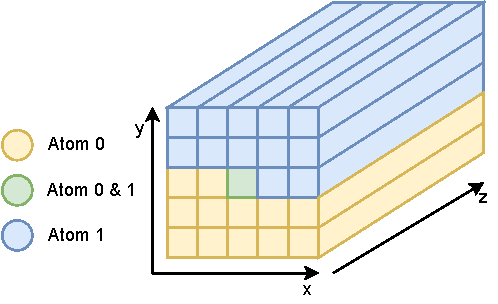
\includegraphics{images/Datenaufteilung_Iteration_2.pdf}
	\caption{Aufteilung des Datenblocks}
	\label{fig:datenaufteilung}
\end{figure}
\begin{figure}
	\center
	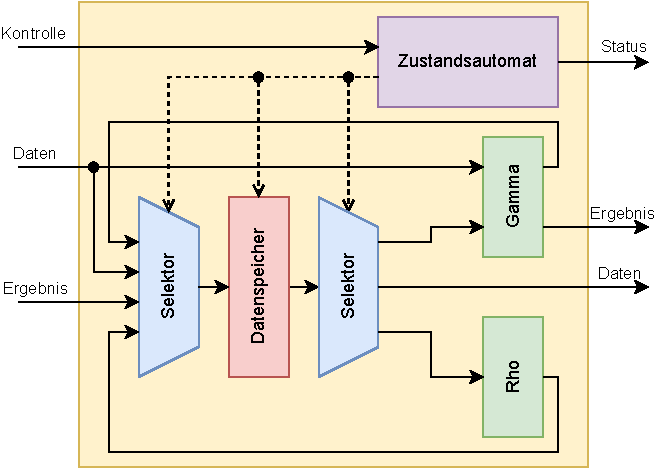
\includegraphics{images/Iteration_2.pdf}
	\caption{Atomaufbau des zweiten Entwurfs}
	\label{fig:aufbau_iteration_2}
\end{figure}

Der Beschleuniger ist in zwei Atome aufgeteilt (Abb. \ref{fig:aufbau_iteration_2}), die jeweils einen Teil des Datenblocks speichern. Beide Atome sind gleich aufgebaut, erst über ein Bit im Kontrollvektor,
den sogenannten \textbf{Atom-Index}, wird festgelegt als welcher Teil des Beschleunigers ein Atom arbeitet. Die Daten sind dabei spaltenorthogonal aufgeteilt, sodass die Lanes 0 bis 12 in Atom 0,
und die Lanes 12 bis 24 in Atom 1 gespeichert werden (Abb. \ref{fig:datenaufteilung}). Die Lane 12 wird dabei absichtlich doppelt gespeichert,
damit beide Atome 13 Lanes speichern, wodurch der gleiche Aufgebaut ermöglicht wird. Jedes Atom speichert somit 13 Lanes aus jeweils 64 Bits, also insgesamt 832 Bits.
Diese Daten werden in einem Block aus FFs gehalten. Über einen Selektor werden aus diesem Datenspeicher die Daten für die Berechnungsblöcke Rho und Gamma sowie für die Kommunikation ausgewählt.
Die Ergebnisse der Berechnungsblöcke sowie die empfangenen Daten werden über einen weiteren Selektor zusammengefügt und wieder im Datenspeicher gespeichert.
Welche Daten von den Selektoren ausgewählt werden und welche im Speicher übernommen werden, bestimmt ein Zustandsautomat. Dieser wird über einen Kontrollvektor von außen gesteuert
und koordiniert die einzelnen Berechnungsschritte und sorgt dafür, dass das Kommunikationsprotokoll befolgt wird.

\subsection{Ablauf einer Berechnung}
\subsubsection{Dateneingabe}
Über den Datenbus werden die Atome mit den Eingabedaten versorgt. Die Eingabe wird entsprechend mit den bereits gespeicherten über ein XOR kombiniert.
Auf diese Weise können der Schwammkonstruktion entsprechend neue Datenblöcke direkt in den Atomen aufgenommen werden ohne,
dass das Ergebis der vorherigen Berechnung erst gelesen werden muss.
\subsubsection{Rho}
Für die Berechnung von Rho werden alle Lanes in einem Atom gleichzeitig in einem Takt wie in einem Schieberegister entsprechend rotiert.
\subsubsection{Gamma}
Die Berechnung von Gamma wird in mehrere Teilschritte aufgeteilt. Atom 0 ist dabei für die Berechnung der Slices 0 bis 31 zuständig und Atom 1
führt die Berechnung für die Slices 32 bis 63 durch. Damit ein neuer Slice berechnet werden kann, muss der vollständige Slice im Atom vorliegen.
Da jeweils 13 Bit schon im eigenen Datenspeicher vorhanden sind, müssen noch 12 Bits aus dem Speicher des anderen Atoms übertragen werden.
Nach der Berechnung muss das Ergebnis in beiden Atomen übernommen werden. Dafür müssen wieder 13 Bits pro Slice übertragen werden.
Um das Kommunikationsprotokoll so einfach wie möglich zu halten und die Ausführungszeit zu minimieren, wird die Berechnung ge-pipelined.
Der 64 Bit breite Voll-Duplex-Kanal zwischen den Atomen wird aufgeteilt in einen 32 Bit breiten Datenkanal und einen 32 Bit breiten Ergebniskanal.
Der genaue Berechnungsverlauf ist noch einmal im Schaubild [Bild Nr] erklärt.
[Schaubild]
\begin{enumerate}
\item Die Daten für Atom 1 werden aus dem Datenspeicher gelesen und an den Datenkanal angelegt.
\item Die Daten für Atom 1 befinden sich im Register des Datenkanals
\item Die Daten für Atom 1 sind am Atom eingetroffen. Gleichzeitig treffen auch die von Atom 1 gesendeten Daten an Atom 0 ein.
Die erhaltenen Daten werden mit den Daten aus dem Speicher von Atom 0 zu vollständigen Slices kombiniert und der Berechnungseinheit bereitgestellt.
\item Die Berechnungseinheit berechnet das Ergebnis und gibt es zurück.
\item Das Ergebnis wird im Datenspeicher übernommen und die Hälfte, die in Atom 1 gespeichert werden soll, wird am Ergebniskanal angelegt.
\item Das Erbebnis im Ergebnisbus befinden sich im Register des Ergebniskanals
\item Das Ergebnis trifft in Atom 1 ein. Gleichzeitig trifft auch das Ergebnis von Atom 1 in Atom 0 ein.
Das erhaltene Ergebnis wird im Datenspeicher übernommen.
\end{enumerate}
Die maximale Anzahl an Slices, die gleichzeitig in einem Atom berechnet werden kann, ergibt sich in diesem Fall aus der stark beschränkten Bandbreite
des Kommunikationskanals. In dem 32 Bit breiten Kanal können maximal zwei 12 Bit bzw 13 Bit Einträge in einem Takt übertragen werden.
Um den gesammten Blockteil zu berechnen, muss die oben aufgeführte Berechnungsabfolge also 16 Mal mit jeweils 2 Slices durchgeführt werden.
Da die Berechnung der 7 Schritte in einer Pipeline durchgeführt wird, beträgt die Berechnungsdauer nicht 16 * 7 = 112 Schritte,
sondern nur 7 + (16 - 1) = 22 Schritte.

\subsection{Bewertung}
Die Ausführungszeit für eine Iteration der modifizierten Rundenfunktion ist wie erwartet etwa um einen Faktor 30 langsamer als die Implementierung der ersten Iteration.
Dies ist wie bereits erklärt hauptsächlich der Aufteilung der Gamma-Funktion in 16 Teilschritte geschuldet, sowie der damit einhergehenden Verzögerung.
Anders jedoch als erwartet, ist die Größe der Atome durch das Aufteilen der Berechnung und des Datenspeichers nicht wie gewünscht gesunken.
Tatsächlich ist der Entwurf mit seinen etwa 4600 LUTs nochmal um gut 37\% größer. Dafür gibt es zwei wesentliche Gründe: den Zustandsautomaten sowie die Speicherkomplexität,
die in der Überlegung für das Design nicht bedacht wurden.
\subsubsection{Zustandsautomat}
Der Zustandsautomat besteht aus einem Iterator, der in jedem Takt hochgezählt wird und anhand dessen die Steuersignale für die anderen Komponenten genertiert werden.
Entgegen der ursprünglichen Annahme, dass seine Größe aufgrund der Einfachheit der Aufgabe vernachlässigbar ist, nimmt er in diesem Design etwa 300 LUTs ein.
Auch wenn sich die konkrete Implementierung noch optimieren lässt, so ist klar geworden, dass die weitere Erhöhung der Berechnungskomplexität mit Bedacht durchgeführt werden muss,
da der Zustandsautomat dadurch nur noch größer wird.
\subsubsection{Schreib- und Lesemuster}
Im ersten Entwurf wird der Wert jedes Bits im Register entweder von der Eingabe oder von der Ausgabe der Rundenfunktion bestimmt.
Im zweiten Entwurf hingegen hängt dieser Wert ab von der Eingabe, des Ergebnisses der Rho-Rotation sowie einem Bit im Ergebnis-Kanal.
Welches Bit aus dem Ergebniskanal für ein Bit im Datenspeicher bestimmt ist, legt der Zustandsautomat und auch der Atom-Index fest.
Diese Auswahlschaltung sowie die Entscheidung, wann genau das Bit im Register überschrieben werden muss (im ersten Entwurf wurden einfach alle Bits in jedem Takt überschrieben, wenn das Kontrollsignal aktiv war),
benötigen schon mehr Platz als die Reduktion der Datenmenge einspart.
Analog ist auch das Lesen der Daten komplizierter geworden. Die Gamma-Funktion sowie der Datenkanal müssen anhand des Zustandsautomaten und des Atom-Indexes aus allen Bits nur ein par auswählen.
\subsubsection{Gamma-Funktion}
Die Gamma-Funktion übernimmt bis auf Rho alle Subfunktionen der Standard-Rundenfunktion. Da die Berechnung auf zwei Atome aufgeteilt ist und auch nicht alle Slices in einem Atom gleichzeitig berechnet werden,
ist die Komplexität der Gamma-Funktion sehr stark geschrumpft, sodass das aktuelle Design nur etwa 70 LUTs benötigt. Eine weitere Optimierung der Gamma-Funktion ist daher auch in weiteren Iterationen nicht mehr nötig.

\subsection{Optimierungsansätze}
Die starke Steigerung der Speicherkomplexität ist das Hauptproblem des Entwurfs und weitere Verbesserungen müssen hier ansetzen, um den Beschleuniger aus die erforderliche Größe reduzieren zu können.
Um die Speicherverwaltung vollständig aus dem Design zu entfernen, hatten wir die Nutzung der BRAM-Blöcke in den Überlegungen des ersten Entwurfs schon einmal erwähnt und uns letztendlich dagegen entschieden,
weil das Festlegen auf einen Tile-orientierten Speicher bedeutet, dass die Rho-Funktion, die eigentlich auf Lanes arbeitet, so implementiert werden muss, dass sie mit Tiles arbeiten kann.
\subsubsection{Transformation der Rho-Funktion}


\subsubsection{BRAM als Datenspeicher}

\subsubsection{Rho-Transformation}

Das Berechnen der Rho-Funktion auf Tile orientierten Daten kann mit Hilfe eines Schieberegisters als Puffer realisiert werden.
Schreibt man alle Rotationen, die größer als 32 Stellen sind, als Rechts-Rotationen um, so müssen in jedem Atom maximal 7 Links- und Rechts-Rotationen durchgeführt werden.
Hier bietet es sich wieder an, die Berechnung in zwei Schritte aufzuteilen. Im ersten Schritt werden die Links-Rotationen berechnet, während die anderen Lanes nicht verändert werden.
Im zweiten Schritt werden dann analog die Rechts-Rotationen durchgeführt. Um das Prinzip zu verdeutlichen, schauen wir uns zuerst die Verarbeitung einer einzelnen Lane an.
Für die Rotation um k Bits einer Lane l mit k < 32, kann die obere Hälfte von l rechts an l angefügt werden.
w = l[63 downto 0] || l[63 downto 32]
rotl(l, k) = w[95 - k downto 31 - k]

Interessant ist, dass diese Berechnung über ein 32 Bit Schieberegister realisiert werden kann.

b[31 downto 0] := l[63 downto 32]
for i in 0 to 63 loop
    r[i] := b[32 - k]
    b := (b >> 1) | (l[i] << 63)
end loop
return r

Mit diesem Vorgehen können die Rotationen berechnet werden, wobei nicht die ganze Lane, sondern immer nur die Hälfte in einem Puffer vorliegen muss.
Da die Berechnung der Rechts-Rotationen analog funktioniert, kann ein Puffer für beide Arten von Rotation verwendet werden.
Des weiteren lässt sich die schleife auch abrollen, womit mehrere Bits auf einmal verarbeitet werden können und natürlich können mit mehreren Puffern auch
mehrere Lanes gleichzeitig rotiert werden. Dabei unterscheiden sich die einzelnen Lanes nur im Index der Auswahl ihrer Ergebnisbits.
Für den konkreten Fall reichen insgesamt 7 Puffer aus. So können im ersten Schritt alle Links- und im zweiten Schritt alle Rechts-Rotationen berechnet werden.
[Schaubild]

\subsubsection{BRAM als Datenspeicher}
Mit dem neuen Ansatz für die Berechnung der Rho-Funktion kann auch der Datenspeicher in den BRAM verschoben werden, da das Problem der unterschiedlichen Ausrichtung der benötigten Eingabedaten behoben ist.
Ein BRAM Block unterstütz dabei bis zu zwei Lese- und Schreibports. Das ist essenziell für die Berechnung der Gamma-Funkion, da durch die Pipeline in jedem Takt sowohl Daten für die eigenen Berechnungen als
auch für die Berechnungen des anderen Atoms gelesen werden müssen und auch die Ergebnisse beider Atome gleichzeitig festgehalten werden.
Da die Gamma-Funktion immer zwei Slices gleichzeitig verarbeitet, bietet sich dieses Format auch für die Speicherstruktur an. So können von jedem Port immer zwei Tiles gleichzeitig adressiert werden.
Da jeder Atom-Contrainer über insgesammt 3 BRAM Blöcke verfügt, können die Ergebnisse der Gamma-Funktion auch in einem anderen BRAM-Block gespeichert werden.
Die Rho-Funktion kann tatsächlich quasi inplace in einem BRAM-Block berechnet werden, da der BRAM read-before-write unterstützt. Wird ein Tile k gelesen und liegt das Ergebnis n Takte später vor,
so kann es an der Stelle k + n gespeichert werden, nachdem im gleichen Takt der alte Slice mit dem Index k + n gelesen wurde.
Das bedeutet, dass beide Ports gleichzeitig Daten für die Berechnung bereitstellen können, sodass immer 4 Tiles gleichzeitig in den Puffer eingelesen werden können.
Auf diese Weise benötigt die Berechnung einer vollständigen Rotation somit theoretisch etwa 8 Takte zum Füllen des Puffers mit den Initialwerten und 16 Takte zum Lesen Schreiben aller Tiles zuzüglich
zu ein paar Verzögerungstakten aufgrund des BRAMs.

\subsubsection{Datenbus}
Da sowohl Gamma als auch Rho in der Zusammenarbeit mit dem BRAM wie es oben beschrieben ist, niemals auf zwei unterschiedlichen BRAM-Blöcken gleichzeitig schreiben oder gleichzeitig lesen,
können die Datenleitungen für die beiden Speicherblöcke zusammengelegt werden.
[Schaubild + Erklärung]


\newpage
\section{Finaler Entwurf}
\subsection{Entwurfsziele}
Mit den vorgestellten Überlegungen soll versucht werden das Design endlich auf die erforderliche Größe zu schrumpfen.
Die Ausführungszeit sollte dabei nicht mehr als bereits in den Überlegungen beschrieben.

\subsection{Aufbau}
\begin{figure}
	\center
	\caption{Atomlayout des Beschleunigers}
	\label{fig:layout_iteration_3}
\end{figure}
\begin{figure}
	\center
	\includegraphics{images/iteration_3.pdf}
	\caption{Aufbau der A-Atome}
	\label{fig:aufbau_iteration_3}
\end{figure}
\begin{figure}
	\center
	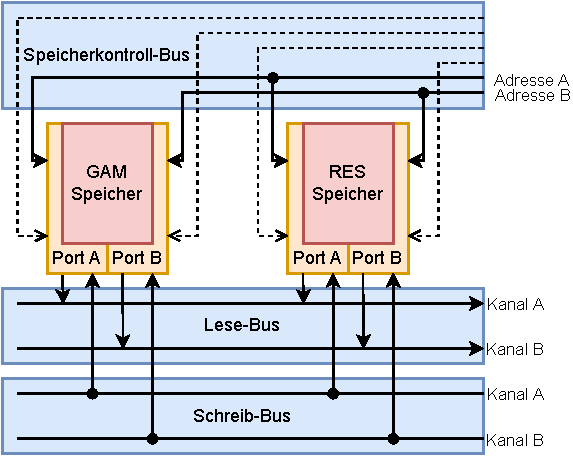
\includegraphics{images/Speicheranbindung.pdf}
	\caption{Speicheranbindung}
	\label{fig:speicheranbindung_iteration_3}
\end{figure}
Der Beschleuniger besteht diesmal aus insgesamt vier Atomen. Die beiden Atome A0 und A1 haben denselben Aufbau und sind für die eigentliche Berechnung der Permutationsfunktion zuständig.
Die Atome B0 und B1 lesen während der Berechnung schon den nächsten Datenblock aus dem externen Speicher ein und konvertieren ihn in Tiles, die dann von den A-Atomen entgegen genommen werden.
Der Beschleuniger besteht wie auch im vorherigen Entwurf aus zwei identischen Atomen, deren Funktionsweise über den Atom-Index definiert wird.
Da der Datenspeicher in den BRAM verschoben wird, müssen die anderen Komponenten so umgebaut werden, dass sie mit dem Interface des BRAM funktionieren.
Dafür werden alle Komponenten sowie der BRAM über einen Speicherbus miteinander verbunden (Abb. \ref{fig:aufbau_iteration_3}).

\subsubsection{BRAM}
Die beiden verwendeten BRAM-Bänke GAM (für Gamma) und RES (für Result) besitzen jeweils zwei Lese-Schreib-Ports, mit denen jeweils ein Tile-Block (bestehend aus zwei benachbarten Tiles) gelesen und auch gleichzeitig geschrieben werden kann (read before write).
Je ein Port ist dabei an den A-Kanal und der Andere an den B-Kanal angeschlossen. 

\subsubsection{Speicherbus}
Der Speicherbus besteht aus drei Segmenten (Abb. \ref{fig:speicheranbindung_iteration_3}). Auf dem Lese-Bus werden Daten aus dem BRAM ausgelesen und den anderen Modulen zur Verfügung gestellt.
Er besteht aus zwei Kanälen, die beide einen Tile-Block breit sind.
Auf dem Schreib-Bus werden Daten von den Berechnungsmodulen und dem Kommunikationsmodul gesammelt und an den BRAM weitergegeben.
Auch dieser besteht aus zwei ein-Tile-Block breiten Kanälen.
Über den Speicherkontroll-Bus werden alle Steuersignale für den BRAM gesammelt. Er besteht aus zwei 7 Bit breiten Address-Vektoren für die beiden Datenkanäle
sowie einem Read-Enable-Signal und einem Write-Enable-Signal für jeden der insgesamt vier Ports.

\subsubsection{Zustandsautomat}
Der Zustandsautomat besteht nicht mehr aus einer Einheit, sondern besteht nun aus einer zentralen Kontrolle sowie spezialisierten Kontrolleinheiten innerhalb der Berechnungseinheiten, angedeutet durch die lila Blöcke.
Die zentrale Kontrolleinheit steuert dabei nur noch den Betriebsmodus des Kommunikationsmoduls und stößt die Abarbeitung in den Berechnungseinheiten an.
Die Kontrolle innerhalb der Berechnungseinheiten bekommt bei Aktivierung die Kontrolle über den Speicherkontroll-Bus und generiert die Steuersignale für die Berechnungseinheit und den Speicher.
Ist die Abarbeitung einer Berechnungseinheit abgeschlossen, wird die Kontrolle wieder an die zentrale Kontrolleinheit übergeben.

\subsubsection{Kommunikationsmodul}
Das Kommunkationsmodul dient zum Datenaustausch zwischen den Atomen sowie zur Kommunikation mit dem externen Speicher, der die Eingabedaten bereitstellt und das Ergebnis entgegennimmt.
Für jede Berechnungseinheit gibt es einen Betriebsmodus, der festlegt, welche Daten von der Berechnungseinheit und dem Speicherbus ausgegeben werden und welche empfangenen Daten an den Speicherbus und die Berechnungseinheit
weitergegeben werden. Dieser Betriebsmodus wird von der zentralen Kontrolleinheit bestimmt.

\subsubsection{Gamma}
Das Gamma-Modul berechnet analog zum Modul aus dem vorherigen Entwurf immer zwei Slices und gibt die entsprechenden Tiles an den Speicher und über das Kommunikationsmodul an das andere Atom aus.
Bis auf die Einführung des Kontrollblocks und einer leichten Anpassung der Schnittstelle ist es identisch zum vorherigen Design. Es nimmt die Eingabedaten aus dem RES-Speicher und schreibt das Ergebnis in den GAM-Speicher

\subsubsection{Rho-Puffer}
\begin{figure}
	\center
	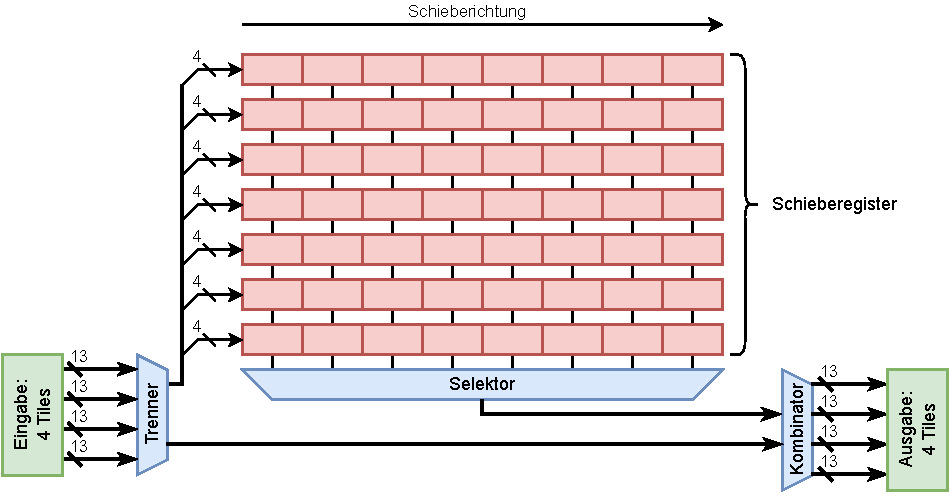
\includegraphics{images/Rho-Aufbau.pdf}
	\caption{Aufbau des Rho-Puffers}
	\label{fig:rho_aufbau_iteration_3}
\end{figure}
Der Rho-Puffer besteht aus sieben 32-Bit-Schieberegistern, die wie in [Ref] verwendet werden, um interativ die Bit-Rotationen zu berechnen (Abb. \ref{fig:rho_aufbau_iteration_3}).
Dazu wird die Berechnung in zwei Schritte unterteilt. Im ersten Schritt werden die Daten aus dem GAM-Speicher gelesen und auf den betrffenden Lanes wird eine Linksrotation durchgeführt, während die anderen Lanes unverändert bleiben.
Das Ergebnis wird im wieder im GAM-Speicher gespeichert. Im zweiten Schritt werden die Daten aus dem GAM-Speicher erneut ausgelesen und diesmal wird auf den übrigen Lanes eine Rechtsrotation durchgeführt. Das finale Ergebnis der Rho-Berechnung
wird dann im RES-Speicher wieder abgespeichert. Es ist die einzige Berechnungseinheit, die keinerlei Kommunikation benötigt und ist daher auch nicht an das Kommunikationsmodul angeschlossen.

\subsubsection{Einlesemodul}
Um das Ergebnis einer Permutation mit einem neuen Datenblock gemäß der Schwammkonstruktion zu kombinieren, müssen die eingelesenen Daten mit den Daten im Ergebnisspeicher mit einem XOR kombiniert werden.
Das Einlesemodul macht genau das und schreibt die kombinierten Daten wieder zurück in den Ergebnisspeicher, sodass erneut die Permutation berechnet werden kann.
Während die neuen Daten eingelesen werden, kann jedoch die eigentliche Berechnung nicht durchgeführt werden. Daher ist es wichtig, dass dieser Schritt so schnell wie möglich abläuft.
Dazu werden die Daten den Atomen direkt als Tiles bereitgestellt, sodass die Einleseeinheit nicht erst die Lanes in Tiles konvertieren muss. Da der Datenblock jedoch in Lanes gespeichert ist,
muss dieser Konvertierungsprozess bereits im Vorhinein irgendwo ausgeführt werden.
Diese Aufgabe übernehmen die Atome B0 und B1. Da die Berechnung der Permutation länger dauert als das Einlesen und die Konvertierung des Datenblocks aus dem externen Speicher,
hat dieser zusätzliche Schritt keinerlei Auswirkung auf die Berechnungsgeschwindigkeit.

\subsubsection{Ergebnismodul}
Zur Ausgabe des 256-Bit Hashes wird das Ergebnismodul verwendet. Es besteht aus einem in FFs implementierten Puffer, der mit den Daten des Ergebnisspeichers gefüllt wird und die Daten so zurück in Lanes konvertiert.
So kann das Ergebnis direkt im richtigen Format ausgegeben werden und im externen Speicher übernommen werden.

\subsection{Berechnung der Permutationsfunktion}
Da die Daten im BRAM nur Slice orientiert als Tiles gespeichert werden und die Eingabedaten aber als Lanes vorliegen, müssen sie erst konvertiert werden.
Diese Konvertierung findet während der vorherigen Berechnung in den B-Atomen statt.
Dabei lesen die B-Atome mehrfach den gesammten Datenblock und puffern immer einen Teil aller Lanes, bis sie sie als vollständige Tiles speichern können.
Dass dabei jede Lane mehrfach eingelesen werden muss, hat keinen Einfluss auf die Ausführunszeit des Beschleunigers, da die Berechnungszeit der modifizierten Rundenfunktion größer ist,
als die Berechnungszeit der Konvertierer und beide Systeme vollständig parallel arbeiten können.
Nachdem ein Block konvertiert wurde und die A-Atome bereit sind, werden die Tiles der Reihe nach über das Kommunikationsmodul von den B-Atomen zum Einlesemodul der A-Atome übertragen
und mit den Daten aus dem RES-Block über ein XOR kombiniert und anschließend wieder in den RES-Block übernommen.
Für die Gamma-Berechnung werden die Slices über den Lesebus aus dem RES-Block gelesen an die Recheneinheit sowie an die Kommunikationseiheit übergeben.
Die Ergebnisse werden anschließend vom Kommunikationsmodul und der Recheneinheit über den Schreib-Bus in den GAM-Block geschrieben.
Anschließend wird die Links-Rotation mit Hilfe des Rho-Puffers durchgeführt. Die Daten werden aus dem GAM-Block über den Datenbus an den Puffer übertragen.
Zuerst wird der Puffer mit den Initialdaten gefüllt, dann werden wie im Abschnitt [Ref] die Tiles nach und nach in den Puffer eingeschoben
und die Erbebnis-Tiles werden über den Schreib-Bus wieder in den GAM-Block übernommen.
Die Rechts-Rotation wird genau so durchgeführt, nur werden dieses Mal die Ergebnisse in den RES-Block geschrieben anstatt in den GAM-Block.
Hier wird auch ein Vorteil des Bus-Designs deutlich: Da beide Blöcke ihre Daten über den Bus empfangen, braucht für die Rechts-Rotation nur das
Write-Enable-Signal verändert werden und die Ergebnisse müssen nicht auf eine andere Eingabe umgeleitet werden.
Die Rho und Gamma Funktionen werden so oft abwechselnd berechnet, bis der Block gemäß der KECCAK-P Funktion verarbeitet wurde.
Danach kann über den Kontrollvektor bestimmt werden, ob entweder der nächste Block eingelesen werden, oder das Ergenis ausgegeben werden soll.
Für die Ausgabe des Ergebnisses werden alle 64 Tiles im Atom A0 vom Ergebnismodul ausgelesen und die ersten 4 Bits in einem FF-Puffer gespeichert.
Als letztes werden diese Ergebnisbits als Lanes ausgegeben und im externen Speicher als Endergebnis gespeichert.

\subsection{Bewertung}


\chapter{Ergebnisse}
Die drei vorgestellten Designs für den Beschleuniger bauen aufeinander auf mit dem Ziel immer mehr Leistung für weniger Platzbedarf einzutauschen.
In diesem Kapitel werden alle Designs miteinander verglichen was sowohl ihre Größe angeht, als auch ihr Leistungspotential.
Das konkrete Ziel dieser Arbeit bestand darin einen Beschleuniger zu entwerfen, der speziell die Anforderungen der i-Core-Architektur erfüllt.
Daher wird in diesem Kapitel hauptsächlich der i-Core als Vergleich herangezogen für die Ausführung von Software-Implementierungen.
Außerdem werden wir uns bei der Untersuchung der Ausführungszeiten auf die KECCAK-p-Funktion beschränken,
da diese den Hauptaufwand darstellt und gerade bei größeren Datenmengen Schritte wie die Initialisierung und das Auslesen des Hashs am Ende vernachlässigbar sind.
Bei Vergleichen zwischen Beschleunigern mit Software-Berechnungen dient immer die Implementierung aus Anhang \ref{cha:anhang1} als Bezug.

\section{Syntheseergebnisse}
\begin{table}
    \centering
    \begin{tabular}{lrrrrr}
    & A-Atome & B-Atome & LUTs & FFs & BRAM Bänke \\
    \hline
    1. Entwurf & 1 & 0 & 3314 & 1845 & 0 \\
    2. Entwurf & 2 & 0 & 4643 & 1865 & 0 \\
    3. Entwurf & 2 & 2 & 1205 & 628 & 2
    \end{tabular}
    \label{tab:synth_ergebniss}
    \caption{Interessante Größen der synthetisierten Designs}
    \small
    Sämtliche Größen beziehen sich auf die A-Atome
\end{table}
In Tabelle \ref{tab:synth_ergebniss} sind die Größen der verschiedenen Beschleunigeriterationen noch einmal zusammengefasst.
Während die ersten beiden Iterationen alle Funktionalitäten in die A-Atomen integrieren, die die tatsächliche Berechnung der KECCAK-p-Funktion durchführen,
benötigt die dritte Iteration noch zwei zusätzliche B-Atome, in denen die Eingabedaten so umgeordnet werden, dass sie in den BRAM der A-Atome geschrieben werden können.
Da in dem dritten Entwurf die Obergrenze von 1600 LUTs für die A-Atome noch nicht erreicht ist, kann diese Funktionalität auch in die Beschleuniger integriert werden.
Je weniger Atome für den Beschleuniger benötigt werden, desto schneller kann der Beschleuniger geladen werden.
Performance-technisch ist es jedoch sinnvoller diese Funktionen zu trennen. Da die A-Atome bei der Berechnung sowohl den BRAM als auch ihre Kommunikationsschnittstelle
voll auslasten, kann die Aufgabe der B-Atome nicht gleichzeitig in den A-Atomen durchgeführt werden. Daher müsste für die Zusammenführung der Atome die Einlese-Phase deutlich verlängert werden.
Für das Verarbeiten großer Datenmengen ist es daher sinnvoll die leicht erhöhte Konfigurationszeit des Beschleunigers in Kauf zu nehmen.

\section{Ausführungszeit}
Zur Bestimmung der Ausführungszeit des Beschleunigers verwenden wir hier die Simulation. Das hat den Vorteil,
dass auch die vorherigen Entwürfe mit verglichen werden können, die zu groß für den i-Core sind.
Da alle Entwürfe statisch sind in ihrer Ausführungszeit, die Abarbeitung eines Blocks also immer die gleiche Zeit benötigt,
liefert diese Herangehensweise genauere Werte als die Zeitmessung es auf dem i-Core tun würde.
Da aller Entwürfe den Betrieb auf dem 50MHz Takt des i-Cores zulassen, können die Taktzahlen direkt miteinander verglichen werden, siehe Tabelle \ref{tab:zeiten_alle_iterationen}.
\begin{table}
    \centering
    \begin{tabular}{lrrr}
        & Berechnungsdauer & Einlesedauer & Gesamtdauer\\
        \hline
        1. Entwurf & 24 Takte & 34 Takte & 58 Takte \\
        2. Entwurf & 509 Takte & 34 Takte & 543 Takte \\
        3. Entwurf & 1968 Takte & 36 Takte & 2004 Takte
    \end{tabular}
    \label{tab:zeiten_alle_iterationen}
    \caption{Ausführungszeiten der verschiedenen Beschleuniger-Entwürfe}
    \small Alle Zeitangaben beziehen sich auf die Abarbeitung eines Datenblocks. Initialisierung und Auslesen des Hashs sind nicht einberechnet.
\end{table}
Die Einlesedauer der Iterationen unterscheidet sich dabei fast gar nicht. In den ersten beiden Entwürfen liegt jede der 17 Lanes aus den Eingabedaten
nacheinander jeweils einen Kontrollschritt, also zwei Takte, an beiden Atomen an und die Atome wählen jeweils die Lanes aus, die sie benötigen
(im ersten Entwurf liest das einzige Atom alle Lanes ein).
Im dritten Entwurf hingegen lesen beide A-Atome gleichzeitig verschiedene Slices, die ihnen von den B-Atomen bereitgestellt werden.
Da in jedem Kontrollschritt jedoch nur jeweils vier Tiles zu je 13 Bits übertragen werden anstatt einer ganzen Lane, werden 16 statt der vorherigen 13 Kontrollschritte benötigt.
Diese Effekte heben sich gegenseitig auf. Eine weitere Optimierung der Einlesezeiten ist auch nicht weiter nötig. Im ersten Entwurf ist sie nicht möglich,
da die Kommunikationsschnittstelle vollständig ausgelastet ist und in den beiden letzten Entwürfen beträgt das Einlesen einen zu kleinen Teil an der gesamten Berechnung.

Die tatsächliche Berechnung hingegen nimmt mit jedem Entwurf deutlich mehr Zeit in Anspruch. Das ist alleine der Sequenzialisierung geschuldet.
Statt wie vorher die gesamte Rundenfunktion in einem Takt abzuarbeiten, werden im zweiten Entwurf Rho in einem Schritt und Gamma/Theta in 16 Schritten für jeweils 2 Slices pro Atom berechnet.
Hinzu kommen noch ein paar Takte durch die Verzögerung zwischen den Atomen, sodass die Berechnung der erweiterten Rundenfunktion im zweiten Entwurf insgesamt 21 Takte benötigt.
Der dritte Entwurf verwendet die gleiche Vorgehensweise für die Berechnung von Gamma/Theta, braucht allerdings drei Takte länger durch die Verzögerung des BRAM
und berechnet außerdem auch Rho sequenziell in 57 Takten. In Tabelle \ref{tab:zeiten_iteration_3} sind die Ausführungszeiten
für die verschiedenen Teilfunktionen im dritten Entwurf noch einmal zusammengefasst.
\begin{table}
    \centering
    \begin{tabular}{lrrr}
    Funktion & Zeit (in Takten) & Iterationen in KECCAK-p & Anteil an KECCAK-p \\
    \hline
    Initialisierung & 18 & - & - \\
    Einlesen & 36 & 1 & 1,8\% \\
    Theta & 24 & 1 & 1,2\% \\
    Gamma & 24 & 24 & 28,74\% \\
    Rho & 57 & 24 & 68,26\% \\
    KECCAK-p & 2004 & 1 & 100\% \\
    Auslesen & 27 & - & -
    \end{tabular}
    \label{tab:zeiten_iteration_3}
    \caption{Ausführungszeiten des finalen Beschleunigers}
\end{table}
Die KECCAK-p-Funktion, für die wir uns eigentlich bei der Berechnung von SHA-3 interessieren, setzt sich zusammen aus dem Einlesen des Datenblocks,
einer Berechnung von Theta, sowie 24 Berechnungen von Rho und Gamma.

\section{Weitere Optimierungsansätze}
Der dritte Entwurf des Beschleunigers erfüllt zwar alle geforderten Voraussetzungen, trotzdem lassen sich noch weitere Verbesserungen vornehmen, um die Leistungsfähigkeit zu erhöhen.
Daher wollen wir uns hier noch ein paar dieser möglichen Optimierungen anschauen.

\subsection{Auslagerung der Ergebniskonvertierung}
Das Ergebnismodul nimmt unnötig viel Platz im Atom ein und ist eigentlich nur deshalb in den A-Atomen enthalten, weil der Platz nicht weiter benötigt wird.
Es lässt sich aber auch in die B-Atome verschieben, die auch die Konvertierung für die Eingabe übernehmen.
So kann noch ein wenig mehr Platz für andere Optimierungen geschaffen werden, die die Berechnungsgeschwindigkeit weiter verbessern.

\subsection{Reduktion auf ein A-Atom}
Die Berechnung wurde ursprünglich auf zwei Atome aufgeteilt, damit die Datenmenge reduziert werden kann, die ein Atom halten muss.
Durch die Verwendung des BRAM für den Datenspeicher fällt dieser Aufwand weg, da der BRAM mehr als genug Platz bereitstellt.
Ein Beschleuniger, der nur ein A-Atom verwendet, bietet vor allem den Vorteil, dass für die Konvertierung der Eingabedaten auch nur ein B-Atom benötigt wird.
Der gesamte Beschleuniger benötigt also nur zwei der fünf Atome. Abhängig vom Anwendungsfall können so auch mehrere kleine Beschleuniger nebeneinander existieren,
ohne dass die Atom-Container zwischendurch rekonfiguriert werden müssen.
Außerdem ist die Berechnung selbst nicht mehr durch die Kommunikationsschnittstelle zwischen den Atomen beschränkt, wodurch weitere Optimierungen möglich werden.
Die Reduktion auf ein A-Atom alleine bringt jedoch keine direkte Leistungsverbesserung. Im Gegenteil, da aktuell beide A-Atome parallel sowohl Rho als auch Gamma berechnen,
würde die Reduktion alleine die Berechnungszeit etwa verdoppeln. Auch das Einlesen der Datenblöcke dauert länger, da der gesamte Block in ein einziges Atom übertragen werden muss,
was wiederum durch die Kommunikationsschnittstelle beschränkt ist. 

\subsection{Erweiterung der BRAM-Schnittstelle}
Aktuell können an einem Port des BRAM immer jeweils zwei Tiles gleichzeitig gelesen und geschrieben werden.
Die Erweiterung der Speicherschnittstelle auf zum Beispiel 4 Tiles erlaubt es,
eine größere Menge an Tiles gleichzeitig für die Berechnung von Rho bereit zu stellen.
Die Rho-Funktion könnte somit doppelt so schnell berechnet werden. Da die Berechnung von Rho mit 57 Takten
etwa 70\% der 81 Takte für die Berechnung der erweiterten Rundenfunktion beansprucht (siehe \ref{tab:zeiten_iteration_3}),
ist nochmal mit einer weiteren Beschleunigung von $S_{WideBRAM} = \frac{81\ Takte}{81\ Takte - (57\ Takte / 2)} \thickapprox 1,54$ zu rechnen.
Die restlichen 30\% der Berechnungszeit für die erweiterte Rundenfunktion werden für die Gamma-Funktion verwendet.
Diese kann durch die Erweiterung der Speicherschnittstelle nicht weiter beschleunigt werden,
da sie die Kommunikationsschnittstelle zwischen den Atomen bereits den limitierende Faktor darstellt.
Unklar ist noch, ob der vorhandene Platz für diese Optimierung ausreicht.

\subsection{Erweiterung des Rho-Puffers}
Möchte man wie oben beschrieben den Beschleuniger auf ein Atom reduzieren, kann auch der Rho-Puffer,
in dem die Bit-Rotationen blockweise auf mehreren Lanes gleichzeitig durchgeführt werden, erweitert werden.
Im aktuellen Entwurf ist das nicht mehr möglich, da genau eine Links- und eine Rechtsrotation auf
etwa jeweils der Hälfte der in den Atomen gespeicherten Lanes durchgeführt werden.
Links- und Rechtsrotationen lassen sich nicht zusammenlegen, was damit zusammenhängt in welche
Richtung die Lanes aus dem Speicher gelesen und geschrieben werden.
Findet jedoch die gesamte Berechnung nur in einem Atom statt, sind für die vollständige Abarbeitung
zwei Links- und zwei Rechts-Rotationen notwendig. Erweitert man den Puffer, sodass jeweils die beiden Links- und die beiden Rechts-Rotationen
zusammengelegt werden können, kann dadurch verhindert werden, dass die Berechnung der Rho-Funktion länger dauert.

\subsection{Auslagerung der Rho-Berechnung}
Es ist zu erwarten, dass die Erweiterung des Rho-Puffers viel zusätzlichen Platz in Anspruch nehmen wird.
Sollte das Atom dadurch die maximale Größe überschreiten, kann eventuell ein Teil der Berechnung von Rho in ein anderes Atom wieder ausgelagert werden.
Aktuell werden in jedem Takt jeweils 4 Bits aus maximal 7 Lanes, also maximal 28 Bit in den Puffer geschrieben und gleichzeitig gelesen.
Dieser Datenverkehr ist über die Kommunikationsschnittstelle durchaus gleichzeitig in beide Richtungen möglich, er kann sogar noch verdoppelt werden,
wenn man auch die BRAM-Schnittstelle wie oben beschrieben erweitert. Jenachdem wie groß diese Konstruktion wird, kann sie auch in das B-Atom integriert werden,
sodass der Beschleuniger trotzdem nur aus zwei Atomen besteht. Das B-Atom würde dann während der Berechnung von Rho mit dem A-Atom zusammenarbeiten und
zwischendurch den nächsten Datenblock einlesen.

\subsection{Erhöhung der Berechnungsfrequenz}
Der Beschleuniger selbst erlaubt eine Taktfrequenz von 200MHz, was in diesem Fall das Maximum für das verwendete FPGA ist. Der i-Core selbst
läuft jedoch nur mit einer Frequenz von 50MHz. Da der Beschleuniger seinen Takt mit dem i-Core teilt, damit die Synchronisierung am einfachsten ist,
läuft er jedoch sehr viel langsamer, als er eigentlich könnte. Verwendet man einen Takt von 200MHz
für die Berechnung der Rho-Funktion, die vollständig in den Atom erfolgt und keinerlei Kommunikation benötigt, erhält man eine Beschleunigung von
$S_{200MHz} = \frac{81\ Takte / 50MHz}{(81\ Takte - 57\ Takte) / 50MHz + 57\ Takte / 200MHz} \thickapprox 2,12$.
Für die Herkunft der genauen Taktzahlen siehe Tabelle \ref{tab:zeiten_iteration_3}. Auch hier kann wieder nur die Rho-Funktion beschleunigt werden,
da die Kommunikation zwischen den Atomen durch den i-core wieder durch den 50MHz-Takt beschränkt ist.

\section{Gemessene Beschleunigung}
Wie bereits erwähnt, sind die entworfenen Beschleuniger strikt deterministisch in der Hinsicht, dass die Dauer der Berechnung immer dieselbe Zeit benötigt.
Daher kann aus den vom Beschleuniger benötigten Takten sowie der Taktfrequenz direkt die Ausführungszeit des Beschleunigers bestimmt werden.
Bei der Software-Berechnung ist das nicht so einfach möglich, da zum Beispiel Speicherzugriffe aufgrund der Speicherstruktur unterschiedliche Ausführungszeiten benötigen.
So kann die Anzahl der auftretenden Cache Misses einen großen Einfluss auf die Berechnungsdauer haben. Auch ist nicht klar, ob wirklich jede Operation des Befehlssatzes
in genau einem Takt ausgeführt werden kann. Durch Datenabhängigkeiten kann es notwendig sein, dass die weitere Abarbeitung auf Ergebnisse vorheriger Instruktionen,
die sich noch in der Pipeline befinden, warten muss. Die beste Möglichkeit zur Bestimmung der Laufzeit der Software-Berechnung ist daher die tatsächliche Zeitmessung.
Diese Messung ist natürlich etwas ungenau, weshalb in 5 Durchläufen jeweils 10.000 Iterationen der KECCAK-p-Funktion durchgeführt werden, woraus dann die mittlere Berechnungsdauer bestimmt wird.
Die Ergebnisse dieser Messungen sowie der berechnete Durchschnitt $\tilde{t}$ sind in Tabelle \ref{tab:software_zeitmessung} aufgeführt.
\begin{table}
    \centering
    \begin{tabular}{lrrrrrr}
        Messung & 1 & 2 & 3 & 4 & 5 & Durchschnitt ($\tilde{t}$)\\
        \hline
        Zeit (s) & 14,505455 & 14,505454 & 14,505463 & 14,505464 & 14,505452 & 14,5054576
    \end{tabular}
    \label{tab:software_zeitmessung}
    \caption{Ausführungszeit der Software-Berechnung}
\end{table}
Aus dieser Messung ergibt sich für eine einzige Berechnung der KECCAK-p-Funktion eine Zeit von
\begin{align*}
    t_{SW} & = \tilde{t}/10000 = 14,5054576 s / 10000 = 1450,54576 \mu s
\end{align*}
Die Ausführungszeit der KECCAK-p-Funktion auf dem finalen Beschleuniger und der daraus resultierende Speedup kann
mit Hilfe der Tabelle \ref{tab:zeiten_iteration_3} aus dem 50MHz-Takt des i-Core wie folgt exakt berechnet werden:
\begin{align*}
    t_{ACC} & = \frac{2004\ Takte}{50 * 10^6Hz} = 0,00004008s = 40,08 \mu s \\
    S_{ACC} & = \frac{t_{SW}}{t_{ACC}}\frac{1450,54576 \mu s}{40,08 \mu s} \thickapprox \mathbf{36,2}
\end{align*}

\section{Theoretische Beschleunigung}
Neben der tatsächlichen Ausführungszeit auf dem i-Core wollen wir uns noch eine andere Metrik anschauen, um den Beschleuniger zu bewerten.
Dazu betrachten wir die Anzahl an elementaren Operationen, die die Software auf einem virtuellen System benötigt, um die KECCAK-p-Funktion zu berechnen.
Als elementare Operationen zählen dabei Instruktionen, von denen man erwarten kann, dass sie von jedem modernen Prozessor in jeweils einem Takt berechnet werden können.
Als solche Instruktionen zählen in diesem Fall XODER, UND, ODER, NEGATION (NEG), das Kopieren, eine Rotation um ein Bit nach links (ROL) sowie ein Bitshift variabler Länge.
Weiter unterschieden werden muss allerdings zwischen 32-Bit- und 64-Bit-Operationen. In der Tabelle \ref{tab:software_instruktionen} ist
die Anzahl der jeweils benötigten 64-Bit-Operationen aufgeführt, die für die einzelnen Teilfunktionen von KECCAK-p benötigt werden, die sich aus insgesamt 24 Runden zusammensetzt.
Die Anzahl an benötigten 32-Bit-Operationen ist dann doppelt so groß. Wie auch in der Implementierung in Anhang \ref{cha:anhang1} beschrieben, ist eine 64-Bit-Rotation,
wie sie zum Beispiel von $\rho$ verwendet wird, dabei aus zwei Shifts und einem ODER zusammengesetzt.
Außerdem werden sämtliche Operationen, die nicht direkt zur die für die Ergebnisberechnung dienen,
wie zum Beispiel Zählvariablen oder Indexberechnungen für Felder, ignoriert.
\begin{table}
    \centering
    \begin{tabular}{lrrrrrrrr}
        & XODER & UND & ODER & NEG & Kopie & ROL & Shift & Gesamt \\
        \hline
        Theta & 50 & 0 & 0 & 0 & 0 & 5 & 0 & 55 \\
        Rho-Pi & 0 & 0 & 24 & 0 & 49 & 0 & 48 & 121 \\
        Chi & 25 & 25 & 0 & 25 & 25 & 0 & 0 & 100 \\
        Iota & 1 & 0 & 0 & 0 & 0 & 0 & 0 & 1 \\
        Rnd & 76 & 25 & 24 & 25 & 74 & 5 & 48 & 277\\
        KECCAK-p & 1824 & 600 & 576 & 600 & 1776 & 120 & 1152 & 6648
    \end{tabular}
    \label{tab:software_instruktionen}
    \caption{Instruktionen der Software-Funktionen}
\end{table}
Da wir gefordert haben, dass jede dieser Operationen in jeweils einem Takt berechnet werden soll,
ergibt sich aus der Anzahl der Operationen auch gleich die Anzahl der benötigten Takte.
Auf diese Weise können wir wieder einen Speedup für den Beschleuniger berechnen, indem wir die benötigten Operationen
der Software mit den benötigten Takten des Beschleunigers vergleichen. Hier können auch alle Entwürfe einbezogen werden,
da wir für unsere virtuelle Umgebung keine Begrenzungen für die Größe der Beschleuniger vorgegeben haben und somit der Vergleich auch sinnvoll ist.
In Tabelle \ref{tab:theoretischer_speedup} ist sowohl der theoretische Speedup sowohl bezüglich 32-Bit- als auch 64-Bit-Operationen aufgeführt.
\begin{table}
    \centering
    \begin{tabular}{lrr}
        & 32-Bit-Speedup & 64-Bit-Speedup \\
        \hline
        1. Entwurf & 229,24 & 114,62 \\
        2. Entwurf & 24,49 & 12,25 \\
        3. Entwurf & \textbf{6,63} & 3,32
    \end{tabular}
    \label{tab:theoretischer_speedup}
    \caption{Theoretischer Speedup der verschiedenen Entwürfe}
\end{table}
Dieser theoretische Speedup beschreibt den Faktor, wie viel der tatsächlichen Berechnung der Beschleuniger in jedem Schritt mehr erledigt,
als die Software es im Optimalfall tut. Vergleicht man den theoretischen Speedup mit dem gemessenen Speedup, so stellt man fest,
dass der gemessene Speedup des finalen Entwurfs mit 36,2 um einen Faktor 5,46 größer ist als der theoretische Speedup von 6,63
(wir verwenden hier den 32-Bit-Speedup, da der i-Core eine 32-Bit-Plattform ist). Dieser Faktor beschreibt die gewonnene Geschwindigkeit,
die dadurch entsteht, dass der Beschleuniger keine Kontrollstrukturen wie Schleifen, Speicherzugriffszeiten, oder mehrere Takte für eine Instruktion benötigt.


\chapter{Fazit}
In dieser Arbeit haben wir gezeigt, wie ein Hardwarebeschleuniger für eine rekonfigurierbare Prozessorplattform
wie den i-Core implementiert werden kann, die die starken Anforderungen, besonders was die maximale Größe des Beschleunigers betrifft, erfüllt.
Dazu sind wir von einem monolithischen Design mit sehr hoher Berechnungsgeschwindigkeit ausgegangen und sind
nach und nach durch kleine Änderungen zu einem modularen System gekommen, das zwar eine geringere
Berechnungsgeschwindigkeit besitzt, dafür aber die Anforderungen der Plattform erfüllt.
Für die vorgenommenen Verbesserungen haben wir verschiedene Ansätze diskutiert und damit die weiteren
Entwurfsentscheidungen begründet. Der entstandene Beschleuniger besteht aus insgesamt vier Atomen,
nutzt jedoch den Platz der den einzelnen Atomen zur Verfügung steht, nicht vollständig aus.
Daher haben wir uns noch weitere vielversprechende Verbesserungsmöglichkeiten für die Zukunft überlegt,
die den noch verfügbaren Platz verwenden, um die Berechnungsgeschwindigkeit weiter zu erhöhen.
Als Beispiel sei da die Erweiterung der Speicherschnittstelle genannt, wodurch die Berechnungzeit der
$\rho$-Funktion, die etwa 70\% der gesamten Berechnungszeit beansprucht, nochmal halbiert werden kann.
Am Ende haben wir den aktuellen Beschleuniger mit einer Software-Implementierung verglichen und festgestellt,
das der entworfene Beschleuniger die Berechnung der KECCAK-p-Funktion, welche bei SHA-3 den alleinigen Rechenaufwand darstellt,
um einen Faktor 36 schneller berechnet, als es die Software auf dem i-Core tut. Über eine genauere Untersuchung
der Berechnungsabläufe in der Software können wir schätzen, dass etwa ein Faktor 6 der gemessenen Beschleunigung
durch die veränderte Berechnungsmethode entsteht und ein weiterer Faktor 6 durch Einflüsse wie Kontrollfluss-Strukturen
in der Software und Speicherzugriffe mit langen Zugriffszeiten, durch zum Beispiel Cache Misses, entstehen.

\chapter{Ähnliche Arbeiten}


- Buehner 2022: Implementierung der inferenz für convolutional neural networks
- Kriebel 2009: Entwicklung von Beschleunigeratomen für SHA-1
- Riedlberger 2015: Implementierung der SHA-1 Spezialinstruktion
- Pöppl 2018: Modelling Shallow Water Waves

\chapter{Glossar}
\section{Begriffe}
\begin{tabularx}{\linewidth}{@{}>{\bfseries}l@{\hspace{.5em}}X@{}}
	Atom: & Beschleuniger, oder Teil eines Beschleunigers, der in einen Atom-Container geladen werden kann \\
	Atom-Container: & Programmierbarer Logikblock in einem rekonfigurierbaren Prozessor \\
	Atom-Index: & Laufzeitparameter des Beschleunigers, der die genaue Aufgabe des Atoms bestimmt \\
	Lane: & Ein eindimensionaler 64-Bit langer Ausschnitt aus einem State Array \\
	Slice: & Ein ein Bit breiter vertikaler Ausschnitt aus allen Lanes, insgesamt 25 Bits groß \\
	State Array: & Die dreidimensionale Darstellung des internen Zustandsvektors der KECCAK-p-Funktion \\
	Schwammkonstruktion: & Teil des SHA-3-Algorithmus, siehe \ref{cha:sha3} \\
	Tile: & Die 13 oberen oder 13 unteren Bits eines Slices (es gibt ein Bit, das in beiden enthalten ist)
\end{tabularx}
\newpage
\section{Abkürzungen}
\begin{tabularx}{\linewidth}{@{}>{\bfseries}l@{\hspace{.5em}}X@{}}
	AC: & Atom Conainer \\
	AGU: & Address Generation Unit \\
	BPP: & Bounded Error Probabilistic Polynomial Time \\
	BQP: & Bounded Error Quantum Polynomial Time \\
	BRAM: & Block RAM \\
	CLB: & Configurable Logic Block \\
	DSP: & Digital Signal Processor \\
	FPGA: & Field Programmable Gate Array \\
	IoT: & Internet of Things \\
	LSU: & Load-Store-Unit \\
	LUT: & Lookup Table \\
	SHA: & Secure Hash Algorithm \\
	SI: & Spezialinstruktion \\
	TLM: & Tile Local Memory \\
	VLCW: & Very Long Control Word
\end{tabularx}

\chapter{Symbolverzeichnis}
\input{chapters/symbolverzeichnis.tex}

\chapter{Anhang 1: Softwareimplementierung}
\label{cha:anhang1}
Für Vergleiche zwischen Software-Algorithmen und Hardware-Beschleunigern ist es wichtig, eine möglichst effiziente Software-Implementierung zu verwenden,
um ein aussagekräftigen Ergebnis zu erhalten. Daher wird für alle Vergleiche in Kapitel \ref{cha:ergebnisse} eine fremde Implementierung verwendet,
die viele Optimierungen enthält. Sie wird vom Github-Nutzer \textit{brainhub} \cite{sha3-impl} unter MIT-Lizenz zur Verfühgung gestellt (\ref{fig:keccak_impl_license}).
Im Folgenden sind die interessanten Segmente der KECCAK-p-Funktion aufgelistet, wobei einige Symbole zur besseren Lesbarkeit umbenannt wurden.

\begin{figure}
\lstset{xleftmargin=2em}
\lstset{language=C}
\begin{lstlisting}[label={lst:keccak_impl_license}]
MIT License

Copyright (c) 2020 brainhub

Permission is hereby granted, free of charge, to any
person obtaining a copy of this software and associated
documentation files (the "Software"), to deal in the
Software without restriction, including without limitation
the rights to use, copy, modify, merge, publish,
distribute, sublicense, and/or sell copies of the Software,
and to permit persons to whom the Software is furnished to
do so, subject to the following conditions:

The above copyright notice and this permission notice shall
be included in all copies or substantial portions of the
Software.

THE SOFTWARE IS PROVIDED "AS IS", WITHOUT WARRANTY OF ANY
KIND, EXPRESS OR IMPLIED, INCLUDING BUT NOT LIMITED TO THE
WARRANTIES OF MERCHANTABILITY, FITNESS FOR A PARTICULAR
PURPOSE AND NONINFRINGEMENT. IN NO EVENT SHALL THE AUTHORS
OR COPYRIGHT HOLDERS BE LIABLE FOR ANY CLAIM, DAMAGES OR
OTHER LIABILITY, WHETHER IN AN ACTION OF CONTRACT, TORT OR
OTHERWISE, ARISING FROM, OUT OF OR IN CONNECTION WITH THE
SOFTWARE OR THE USE OR OTHER DEALINGS IN THE SOFTWARE.
\end{lstlisting}
\caption{Lizenz der verwendeten SHA-3-Implementierung}
\label{fig:keccak_impl_license}
\end{figure}

\begin{figure}
\lstset{xleftmargin=2em}
\lstset{language=C}
\begin{lstlisting}[label={lst:keccak_impl_utils}]
static const uint64_t keccak_rount_constants[24] = {
    0x0000000000000001ULL, 0x0000000000008082ULL,
    0x800000000000808aULL, 0x8000000080008000ULL,
    0x000000000000808bULL, 0x0000000080000001ULL,
    0x8000000080008081ULL, 0x8000000000008009ULL,
    0x000000000000008aULL, 0x0000000000000088ULL,
    0x0000000080008009ULL, 0x000000008000000aULL,
    0x000000008000808bULL, 0x800000000000008bULL,
    0x8000000000008089ULL, 0x8000000000008003ULL,
    0x8000000000008002ULL, 0x8000000000000080ULL,
    0x000000000000800aULL, 0x800000008000000aULL,
    0x8000000080008081ULL, 0x8000000000008080ULL,
    0x0000000080000001ULL, 0x8000000080008008ULL
};

static const unsigned keccak_rho_distances[24] = {
    1, 3, 6, 10, 15, 21, 28, 36, 45, 55, 2, 14,
	27, 41, 56, 8, 25, 43, 62, 18, 39, 61, 20, 44
};

static const unsigned keccakf_pi_indices[24] = {
    10, 7, 11, 17, 18, 3, 5, 16, 8, 21, 24, 4, 15,
	23, 19, 13, 12, 2, 20, 14, 22, 9, 6, 1
};

#define ROTL(x, y) \
	(((x) << (y)) | ((x) >> ((sizeof(uint64_t)*8) - (y))))
#endif
\end{lstlisting}
\caption{Konstanten und Hilfsfunktionen der KECCAK-p-Implementierung}
\label{fig:keccak_impl_utils}
\end{figure}

\begin{figure}
\lstset{xleftmargin=2em}
\lstset{language=C}
\begin{lstlisting}[label={lst:keccak_impl}]
static void keccak_p(uint64_t stateArray[25]) {
  int i, j, round;
  uint64_t temp, buffer[5];
  #define KECCAK_ROUNDS 24

  for(round = 0; round < KECCAK_ROUNDS; round++) {

    /* Theta */
    for(i = 0; i < 5; i++)
      buffer[i] = stateArray[i] ^ stateArray[i + 5]
	    ^ stateArray[i + 10] ^ stateArray[i + 15]
        ^ stateArray[i + 20];

    for(i = 0; i < 5; i++) {
      temp = buffer[(i + 4) % 5] ^ ROTL(buffer[(i + 1) % 5], 1);
      for(j = 0; j < 25; j += 5)
        stateArray[j + i] ^= t;
    }

    /* Rho Pi */
    temp = stateArray[1];
    for(i = 0; i < 24; i++) {
      j = keccakf_pi_indices[i];
      buffer[0] = stateArray[j];
      stateArray[j] = ROTL(t, keccak_rho_distances[i]);
      temp = buffer[0];
    }

    /* Chi */
    for(j = 0; j < 25; j += 5) {
      for(i = 0; i < 5; i++)
        buffer[i] = stateArray[j + i];
        for(i = 0; i < 5; i++)
          stateArray[j + i] ^= (~buffer[(i + 1) % 5])
                               & buffer[(i + 2) % 5];
    }

    /* Iota */
    stateArray[0] ^= keccak_round_constants[round];
  }
}
\end{lstlisting}
\centering
\caption{Implementierung der KECCAK-p-Funktion}
\small Mit dieser Implementierung wurden die Tests in Kapitel \ref{cha:ergebnisse} durchgeführt.
\label{fig:keccak_impl}
\end{figure}




\chapter{Template Stuff that is still here}

\section{Some Template Comments}
\label{sec:comments}

\begin{outline}
  \1 It is recommended to use one sentence per line of the latex source code.
  That is a good compromise between (i) `diffs' when using repositories, and (ii) forward-/backward search between latex source code and pdf output.
  \1 Note that you can have multiple refs in the same \textbackslash cref block (e.g., \cref{sec:motivation,sec:comments,sec:statement,sec:results,fig:popcount}), but there must not be spaces after the commas.
  \1 Note that you should use \textbackslash Cref (upper-case C) at the beginning of a sentence and \textbackslash cref (lower-case c) in the middle of a sentence.
  They are defined differently, such that the upper-case C version does not use abbreviations (which is recommended for the beginning of a sentence), e.g., \cref{eq:node} vs. \Cref{eq:node}.
  \1 You can use the outline environment to collect itemized points before actually writing your text.
    \2 It helps structuring your ideas by simplifying indentation of items
    \3 Like here.
\end{outline}


\section{Problem Statement}
\label{sec:statement}

Based on a partitioning $P \subset 2^V$, i.e., $p_i, p_j \in P, p_i \ne p_j \Rightarrow p_i \cap p_j = \emptyset, \bigcup\limits_P = V$, an equivalence relation $\sim_P$ as well as the partition graph $G_P$ are defined as follows:
\begin{align}
  \sim_P &= \{(v_1,v_2) \in V | \exists p \in P: v_1\in p \wedge v_2 \in p\}\\
  G_P &= (V_P, E_P) = (V/\sim_P, \{ ([v_1]_{\sim_P}, [v_2]_{\sim_P}) |\: (v_1,v_2) \in E \})
  \label{eq:node}
\end{align}



\section{Results}
\label{sec:results}

Following is the discussion of obtained results.

\begin{figure}[ht]
  \center
  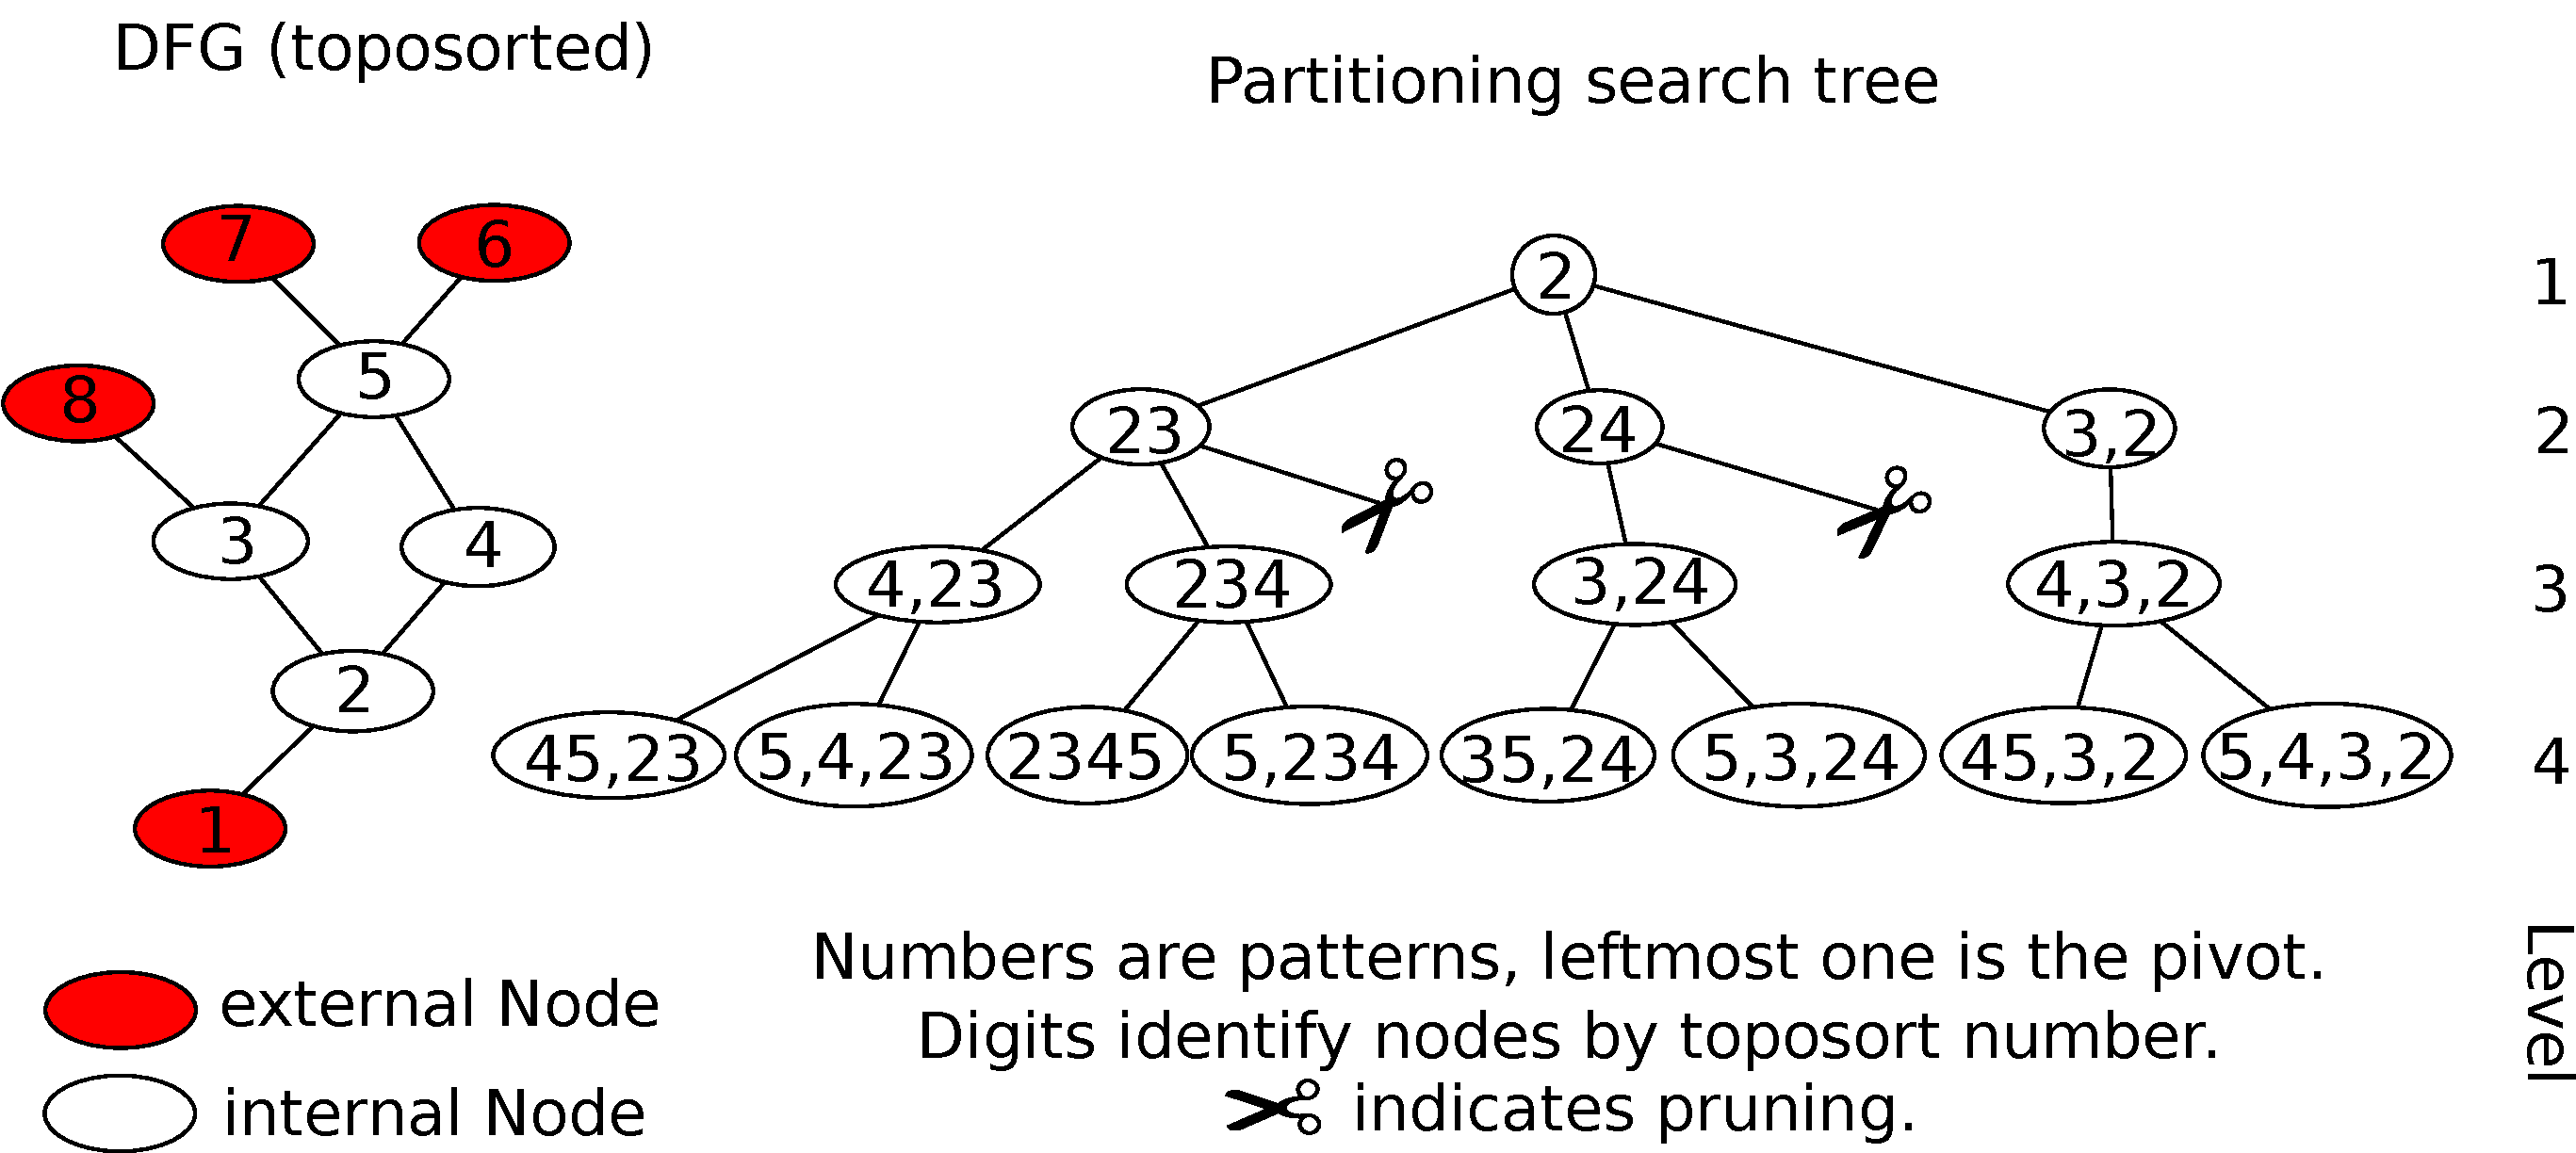
\includegraphics[scale=0.33]{searchtree.pdf}
  \caption{Topologically sorted DFG along with the complete search tree of the partition enumeration algorithm.}
  \label{fig:searchtree}
\end{figure}



\begin{table}
  \centering
  \begin{tabular}{lrrrr}
                &   types  &      types  &   atoms  &      atoms  \\
    SI          &  manual  &  generated  &  manual  &  generated  \\
    \hline
    htfour      &       1  &          4  &       8  &         81  \\
    satdfour    &       3  &          8  &      16  &        104  \\
    dctfour     &       2  &          9  &      12  &         90  \\
    sadsixteen  &       1  &          4  &      64  &        255  \\
  \end{tabular}
  \caption{Comparison of generated SI graphs vs. hand-crafted ones.}
  \label{tab:manualeval}
\end{table}


\begin{figure}
\lstset{language=C}
\begin{lstlisting}[label={lst:popcount}]
uint32_t popcount_a(uint32_t x)
{
  x -= ((x >> 1) & 0x55555555);
  x = (x & 0x33333333) + ((x >> 2) & 0x33333333);
  x = (x + (x >> 4)) & 0x0f0f0f0f;
  x += x >> 8;
  x += x >> 16;
  return x & 0x3f;
}
\end{lstlisting}
\caption{C-Code from \cite{warren2003hacker} to compute the number of set bits of a 32-bit value.}
\label{fig:popcount}
\end{figure}

